% Chapter 1

\chapter{Adversarial Networks Training} % Main chapter title
\label{Chapter5} % For referencing the chapter elsewhere, use \ref{Chapter1} 

Now that we built our dataset, we have the data we need to proceed with the adversarial training of our pipeline.

It is once again important to place this chapter in the context of our data pipeline, as we introduced it in section~\ref{sec:datapipeline} and as we showed it in figure~\ref{fig:pipeline}. The dataset we just created is composed of policies (which are just tables or 2D matrices).  More specifically we have 3,827 such policies, corresponding to all the 3,827 different valid map configurations of our environment, \code{RandomisedFrozenLake}. We split the dataset in a training subset (80\%) of the total number of policies, and the test subset (the remaining 20\%).

In section~\ref{sec:gan} we introduced Generative Adversarial Networks, detailing their vanilla architecture, as they were introduced by \citeauthor{goodfellow2014generative}. We now build off of this architecture to build a GAN architecture for policy generation.

In this section we present such architecture, explain the design decisions that were involved in configuring it, and describe the process of training it in an adversarial manner. We also provide a detailed breakdown of the generator and the discriminator's deep neural networks.

The input to our Policy GAN will only be the training subset of the policies we trained with Q-learning. In this way, we hope to be able to model, through our GAN, a distribution on these policies such that we can capture knowledge that we can transfer to other unseen tasks.
These unseen tasks are exactly the ones corresponding to the map configurations of the test substed, and we therefore do not include those test policies as our input to our GAN.

%----------------------------------------------------------------------------------------

\section{Policy GAN}
In figure~\ref{fig:PolicyGAN} we show the architecture of our Policy GAN.
We already described most of the details involved when training GANs in section~\ref{sec:gan}. 

Training a GAN is an iterative process that runs for a set amount of epochs (an epoch is one full training cycle on the training set).
At each iteration, the mini-batch inputs to the discriminator \code{D} are taken from both the real data sampled from the training data (in our case policies from the training set that we created in chapter~\ref{Chapter4}), and the samples generated by the generator.
Given \code{D}'s prediction, we then apply a gradient-based optimisation method to update both \code{D}'s and \code{G}'s parameters.

Building neural net architecture that work well in practice generally involves finding and tuning many parameters and making several design decisions that make the issue not trivial. In the following subsections, we introduce such decisions and hyperparameters choice with the aim of allowing reproducibility of our results.

%TODO Graph losses Generator Discriminator

\begin{figure}
\centering
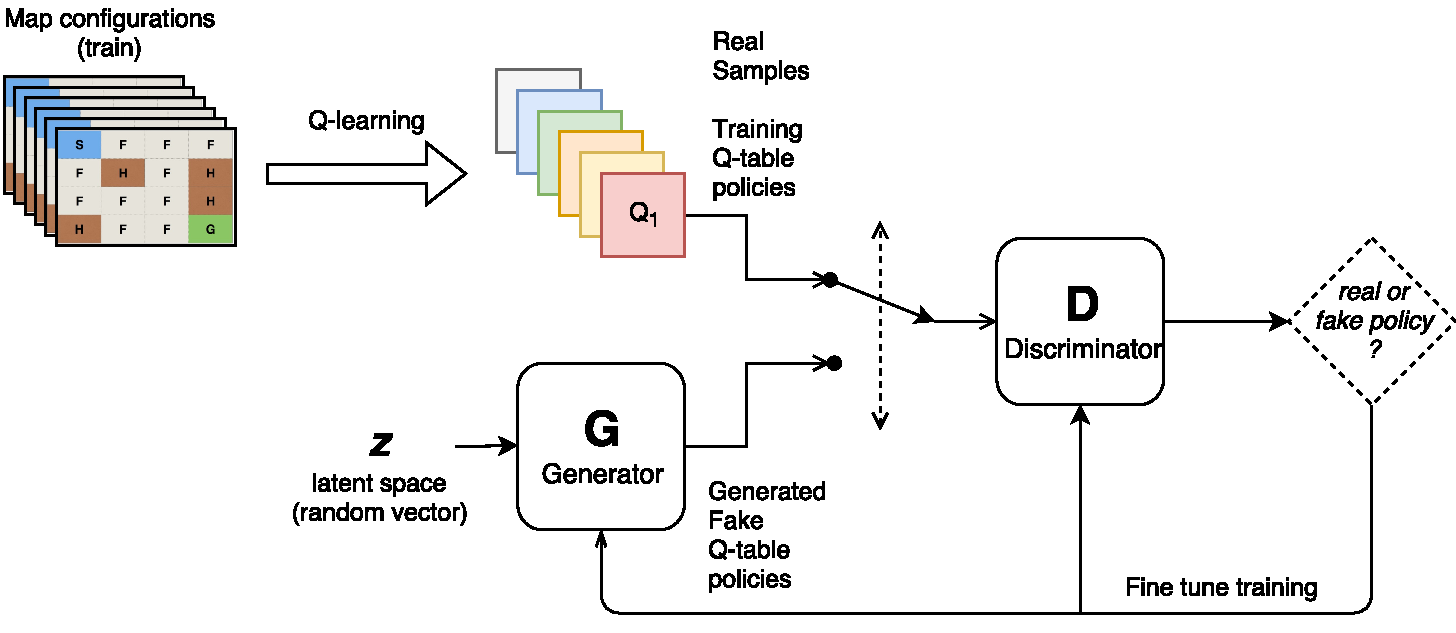
\includegraphics[width=15cm]{Figures/PolicyGAN}
\caption{Our Policy GAN architecture}
\label{fig:PolicyGAN}
\end{figure}

\subsection{Gradient descent optimisation}
Learning rates and gradient descent optimisations algorithms have historically been among the trickiest hyperparameters to set, as they drastically influence the final results, perhaps more than all other hyperparameters.

Gradient descent \citep{lemarechal2012cauchy}, a seminal approach to optimisation that dates back to Cauchy a few centuries back, still proves relatively successful in many machine learning applications.
Since then, a lot of work has been put in devising algorithms that have adaptive learning rates and that lead to faster convergence. In our design, we specifically explored two such adaptive learning rates algorithms: RMSProp \citep{hinton2012neural} and Adam \citep{DBLP:journals/corr/KingmaB14}

Both perform local optimisation with different techniques and metrics that are constructed from the history of previous interactions.

RMSProp (algorithm \ref{alg:RMSProp}) is a modification of the AdaGrad optimiser \citep{duchi2011adaptive}, that modifies the gradient accumulation into a moving average that is exponentially weighted.

Adam (algorithm \ref{alg:Adam}) is best described as a combination of RMSProp and Stochastic Gradient Descent (SGD) with momentum \citep{sutskever2013importance}. Momentum accelerates SGD by multiplying the learning rate by a parameter that increases as we go towards the right direction in the gradient update.

\begin{algorithm}[ht]
\begin{algorithmic}
   \STATE {\bfseries Require:} Global learning rate $\epsilon$, decay rate $\rho$
   \STATE {\bfseries Require:} Initial parameter $\theta$
   \STATE {\bfseries Require:} Small constant $\delta$, usually $10^{-6}$, used to stabilize division by small number
   
   \STATE Initialize accumulation variables $\boldsymbol{r=0}$
   \WHILE{stopping criterion not met}{}
   \STATE Sample a minibatch of $m$ examples from the training set $\{x^{(1)},...,x^{(m)}\}$ with corresponding targets $y^{i}$.
   \STATE Compute gradient: $\boldsymbol{g \leftarrow \frac{1}{m}\nabla_\theta \sum_i L(f(x^{(i)}; \theta), y^{(i)}).}$
   \STATE Accumulate squared gradient: \\ $\boldsymbol{r \leftarrow \rho r + (1 - \rho) g \odot g}$
   \STATE Compute parameter update: $\boldsymbol{\Delta\theta = -\frac{\epsilon}{\sqrt{\delta+r}} \odot g.}$ ($\frac{1}{\sqrt{\delta+r}}$ applied element-wise)
   \STATE Apply update: $\boldsymbol{\theta \leftarrow \theta + \Delta \theta}$
   \ENDWHILE
\end{algorithmic}
  \caption{RMSProp algorithm}
  \label{alg:RMSProp}
\end{algorithm}


\begin{algorithm}[ht]
\begin{algorithmic}
   \STATE {\bfseries Require:} Step size $\epsilon$ (Suggested default: 0.001)
   \STATE {\bfseries Require:} Exponential decay rates for moment estimates, $\rho_1$ and $\rho_2$ in $[0,1)$. (Suggested defaults: 0.9 and 0.999 respectively)
   \STATE {\bfseries Require:} Small constant $\delta$ used for numerical stabilisation (Suggested default: $10^{-8}$)
   \STATE {\bfseries Require:} Initial parameters $\theta$
   
   \STATE Initialise 1st and 2nd moment variables $\mathbf{s=0, r=0}$
   \STATE Initialise time step $t=0$
   \WHILE{stopping criterion not met}{}
   \STATE Sample a minibatch of $m$ examples from the training set $\{x^{(1)},...,x^{(m)}\}$ with corresponding targets $y^{i}$.
   \STATE Compute gradient: $\boldsymbol{g \leftarrow \frac{1}{m}\nabla_\theta \sum_i L(f(x^{(i)}; \theta), y^{(i)}).}$
   \STATE $t \leftarrow t + 1$
   \STATE Update biased first moment estimate: $\boldsymbol{s \leftarrow \rho_1 s + (1-\rho_1) g}$
   \STATE Update biased second moment estimate: $\boldsymbol{r \leftarrow \rho_2 r + (1-\rho_2) g \odot g}$
   \STATE Correct bias in first moment: $\boldsymbol{\hat{s} \leftarrow \frac{s}{1-\rho_1^t}}$
   \STATE Correct bias in second moment: $\boldsymbol{\hat{r} \leftarrow \frac{r}{1-\rho_2^t}}$
   \STATE Compute update: $\boldsymbol{\Delta \theta = -\epsilon \frac{\hat{s}}{\sqrt{\hat{r}} + \delta}}$
   \STATE Apply update: $\boldsymbol{\theta \leftarrow \theta + \Delta \theta}$
   \ENDWHILE
\end{algorithmic}
  \caption{Adam algorithm}
  \label{alg:Adam}
\end{algorithm}

Like in most applications involving deep learning, there is no definite way to see which approach would yield the best results without going through the whole training process.

We therefore empirically experiment with each of these approaches to see which choice is more suitable to our data distribution and yields the best results. "Best", in our case, is seen in the context of both the Generator network and the Discriminator network.

We look for an optimisation technique that leads to stable costs for both networks. In most deep learning problems, convergence of the cost function is limited to one single neural network. In adversarial architectures like GANs, or architectures with multiple deep neural networks like Variational Autoencoders (VAE), or Actor-Critic networks, convergences of the model is not a property that we can trivially evaluate \citep{kingma2013auto, grondman2012survey}.

We look for an asymptotic behaviour that has both networks converge to an optimum, without having one network prevail over the other. For example, we could have a Discriminator that produces perfect predictions after a few epochs of training, but that is a meaningless result if the Generator is not able to produce results that can "fool" the discriminative model.

The overall cost of the architecture, in short, must take into account both components:

\[\min_{G} \max_{D} V(G, D) = \mathbb{E}_{x\sim p_{data}(x)}[log D(x)] + \mathbb{E}_{z \sim p_{g}(z)}[log(1-D(G(z)))] \]

With both RMSProp and Adam we obtain much better convergence compared to vanilla SGD. While do not notice a noticeable difference between these two results, having adaptive learning rates clearly helps convergence for both models.

After optimising our hyperparameters with grid-search, our final optimal optimisation is the following: \\\\
Adam, step size $\epsilon = 0.0002$, exponential decay rates $\rho_1 = 0.5$, $\rho_2 = 0.999$.

%TODO Comparisons of design decisions

\subsection{Hidden layers}



%----------------------------------------------------------------------------------------


\section{Generator}
Figure~\ref{fig:Generator} shows the 

\subsection{Activation functions}

\subsection{Batch Normalisation}
Batch Normalisation \citep{DBLP:journals/corr/IoffeS15} is a technique that improves stability and performance of neural networks by normalising the inputs of each layer such that they have a mean output activation of zero and standard deviation of one. Benefits of using batch normalisation include faster training time (i.e. faster convergence to optimal model). This also allows higher learning rates and weight initialisation won't be as critical.

We first compute the mean and variance of each hidden unit activation across the minibatch (size $M$):
\begin{gather*}
\mu_i \leftarrow \frac{1}{M} \sum_{m=1}^{M}u_i^m \\
\sigma_i^2 \leftarrow \frac{1}{M} \sum_{m=1}^{M}(u_i^m - \mu_i)^2
\end{gather*}

The result of doing batch normalisation will then be:
\begin{gather*}
u_i = w_ix \\
\hat{u_i} = \frac{u_i-\mu_i}{\sqrt{\sigma_i^2 + \epsilon}} \\
z_i = \gamma_i\hat{u_i}+\beta_i = \text{batchNorm}({u_i})
\end{gather*}

where $\gamma$ and $\beta$ are parameters updated with gradient descent that will scale and shift the normalised activations.


\begin{figure}
\centering
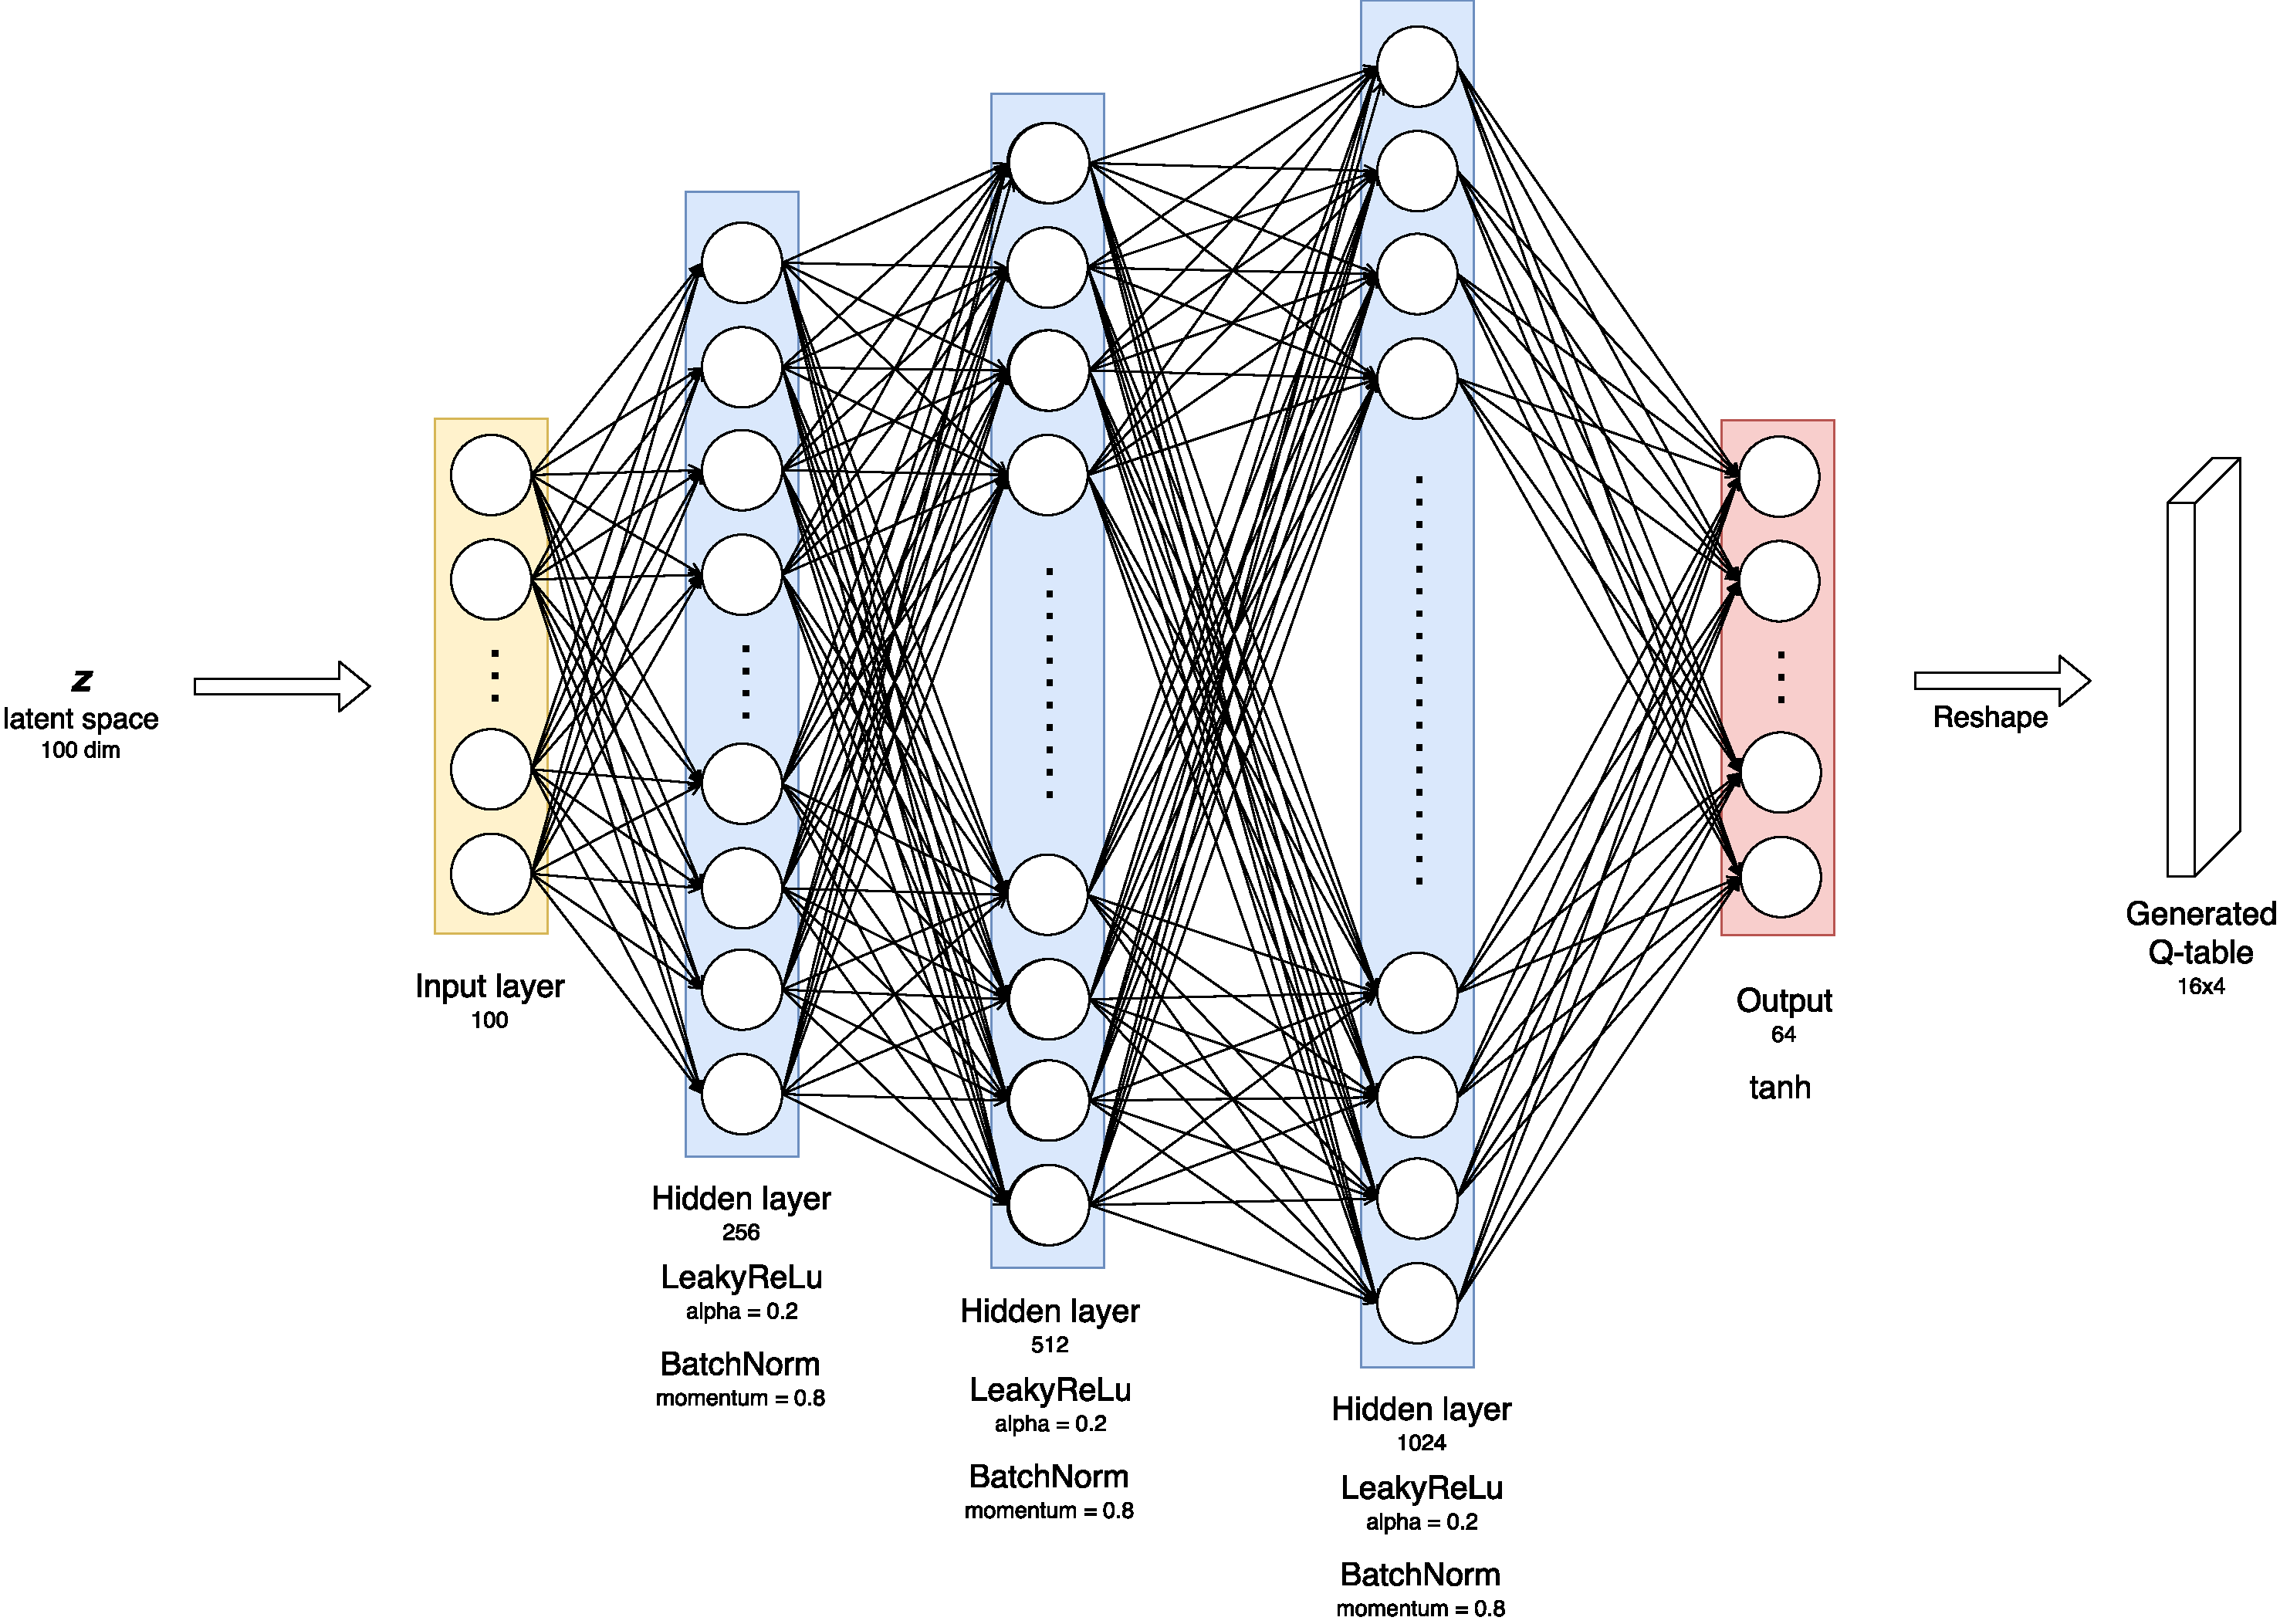
\includegraphics[width=15cm]{Figures/Generator}
\caption{Architecture of the Generator network}
\label{fig:Generator}
\end{figure}

%----------------------------------------------------------------------------------------

\section{Discriminator}
\begin{figure}
\centering
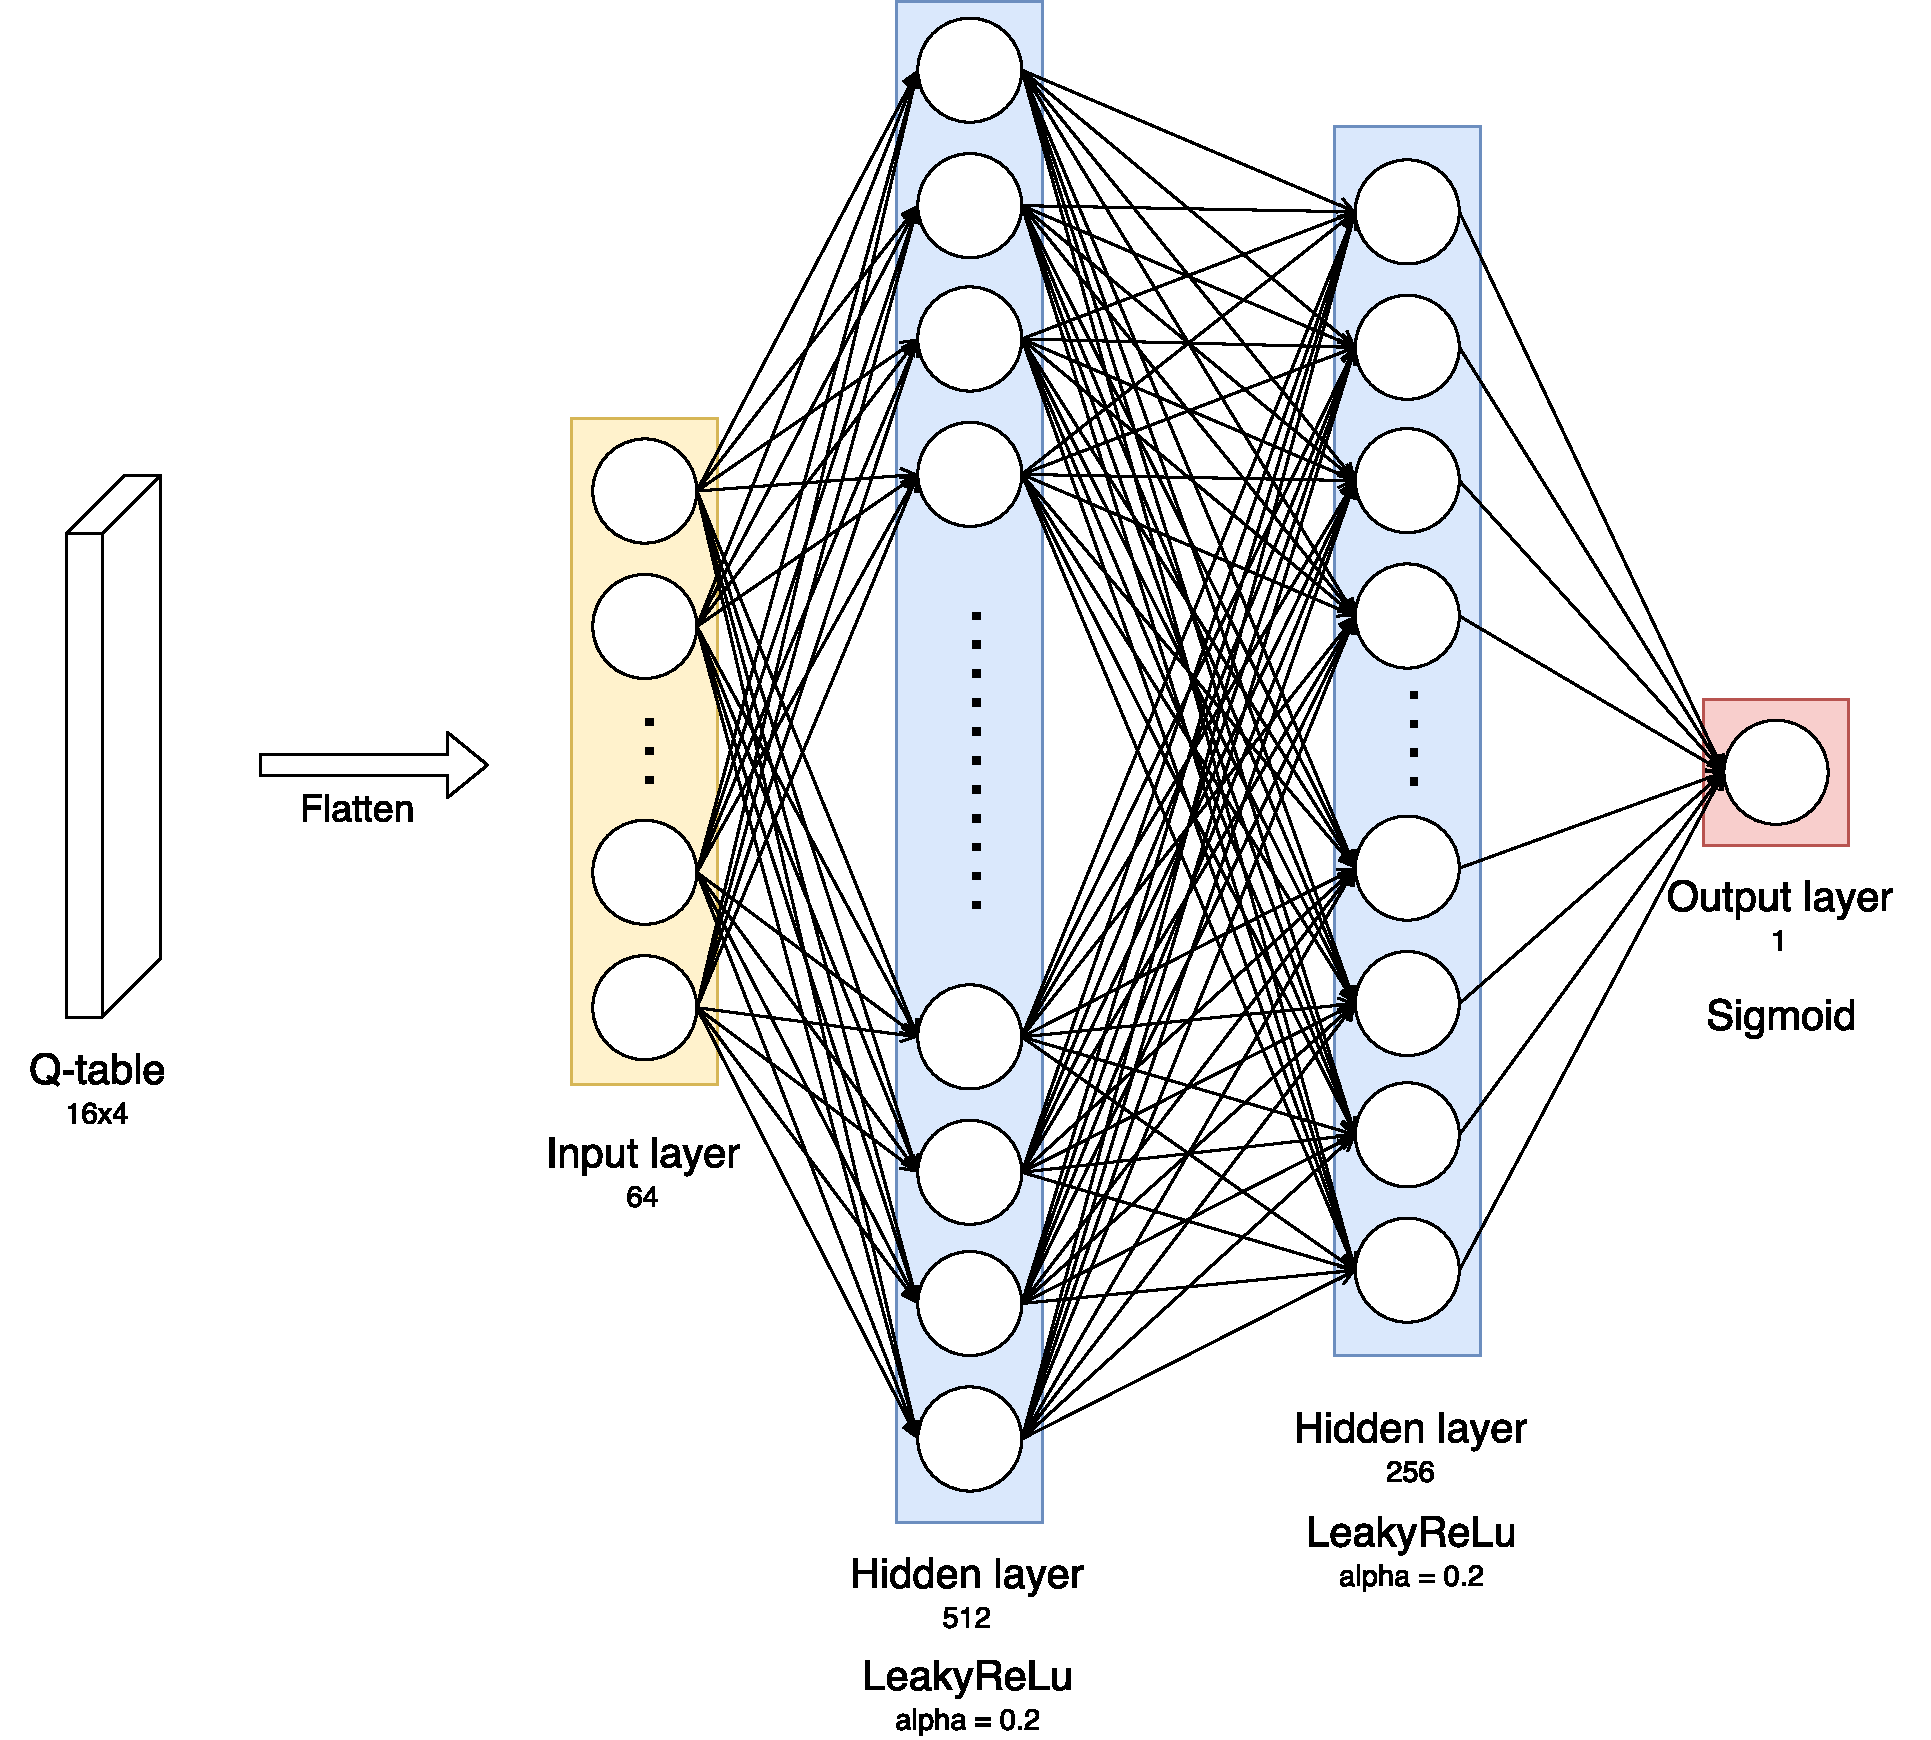
\includegraphics[width=10cm]{Figures/Discriminator}
\caption{Architecture of the Discriminator network}
\label{fig:Discriminator}
\end{figure}